\chapter{Introduction}
\label{chap:introduction}


\emph{Data Science} is a very vibrant field of research that has been gaining more and more interest in the past decade, both in academy and industry. 
\begin{figure}
\centerline{
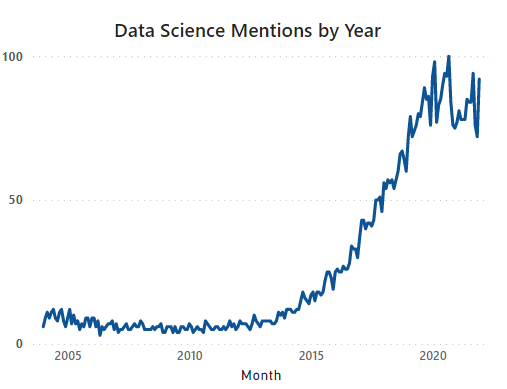
\includegraphics[width=0.5\textwidth]{figures/DataScience/trend_ds.png}
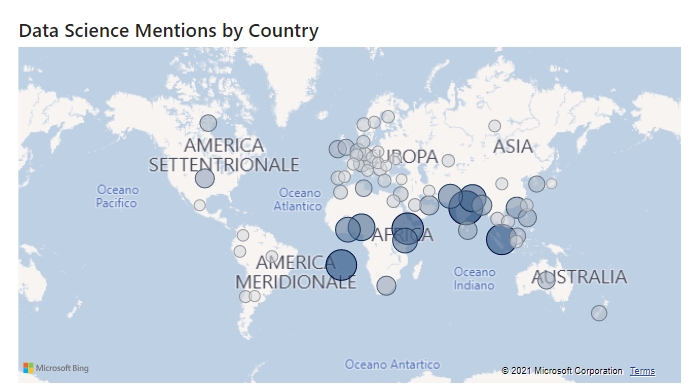
\includegraphics[width=0.5\textwidth]{figures/DataScience/map_ds.png}
}
\caption{
\textbf{Data Science Google searches}. Trends and geolocalization of Google searches of "data science" from 01/01/04 to 06/12/21.
} 
\label{fig:GoogleTrendsDS}
\end{figure}
That much so that it was awarded the title of \textquote{sexiest job of the 21st century} \cite{davenport2012sexiest}, and only American universities counted 78 data science programs in 2020 \cite{zhang2021data}.
However, the discussion over data science's essence has a long history, and multiple definitions have been proposed over the years \cite{donoho201750years}.
Although researchers and practitioners are yet to reach a complete agreement on its exact meaning  \cite{ASA2015statement}, \emph{five} common pillars can be identified by the various definitions.
First, \textbf{multidisciplinarity} is indisputably a key element stressed in every definition of data science. 
Second, as the name suggests, the \textbf{focus on data} and adequate techniques to manage and process them is inevitably an essential aspect.
Third, data science requires adopting suitable \textbf{analytical models} to transform data into knowledge.
Fourth, the \textbf{computing infrastructure} that is necessary to run data analysis timely and efficiently. 
Fifth, a compelling \textbf{visualization and communication} of results that are simple enough to speak to a heterogeneous and non-technical audience, yet comprehensive of all relevant details to convey meaningful insights.

Inspired by these principles, this thesis describes the development of two data science projects and how the five pillars above are declined in practice.


\paragraph{Structure of the Thesis}

After an initial definition of the discipline of \emph{Data Science}, this thesis is organized as follows.

\Cref{chap:historyDS} draws a historical reconstruction of the evolution of the concept of data science over time, trying to clarify what this subject is all about and set an unambiguous reference framework. 

\Cref{partI} explores in greater details the work presented in \citeA{morelli2021cresunet}. In particular, \Cref{chap:partI_intro} describes the technique of microscopic fluorescence and its application to life science and biology experiments. The task of counting objects in digital images is then presented, and some relevant available literature is reviewed.
\Cref{chap:partI_dataset} describes the \textbf{Fluorescent Neuronal Cells} dataset \cite{clissa2021fluocells}, focusing on data acquisition, data annotations, and peculiar characteristics and challenges. 
In \Cref{chap:partI_methods}, the \textbf{cell ResUnet (c-ResUnet)} \cite{morelli2021cresunet} model is introduced and compared with some alternative architectures. Also, three experimental settings are detailed, which are then used for testing competing architectures through ablation studies.
In \Cref{chap:partI_results}, the performances achieved by the proposed approaches are evaluated both quantitatively and qualitatively.
Finally, \Cref{chap:partI_conclusions} summarizes the main findings of the study and discusses possible extensions.

\note[Luca][notesyellow]{TO BE COMPLETED WITH WHOLE STRUCTURE.}

\section{History of Data Science}
\label{chap:historyDS}

The first trace of this debate dates back to \cite{tukey1962future}, where Tukey uses the term \emph{data analysis} to indicate a discipline with the connotations of a \emph{science} and which is \textquote{defined by a ubiquitous problem rather than by a concrete subject}. 
Tukey's description incorporates many aspects seemingly tied closely to applied statistics: 
\begin{displayquote}
procedures for analyzing data, techniques for interpreting the results of such procedures, ways of planning the gathering of data to make its analysis easier, more precise or more accurate, and all the machinery and results of (mathematical) statistics which apply to analyzing data.
\end{displayquote}
Nevertheless, the extent Tukey attributes to data analysis is broader than its philological meaning, as it comprises all of statistics and embeds it in a larger entity \cite{huber2012data, donoho201750years}.
Indeed, Tukey himself sets the boundaries between data analysis and statistics in their respective binding to the strict formalism of mathematics.

In fact, he appeals for a looser attachment to mathematical foundations and suggests focusing on actionable insights rather than theory.
 - scope and usefulness over security
 - inadequate evidence shall suggest right answers
 - maths as judgment rather than proof
 
Finally, Tukey identified four driving forces in the emerging data analysis science:
Four major influences act on data analysis today:
1. The formal theories of statistics
2. Accelerating developments in computers and display devices
3. The challenge, in many fields, of more and ever larger bodies of data
4. The emphasis on quantification in an ever wider variety of disciplines

Despite being released 60 years ago, Tukey's description is incredibly modern and well depicts many activities currently under the umbrella of what we refer to as data science today.
Nonetheless, researchers and practitioners are yet to reach a complete agreement on its definition.

By and large, bla bla bla...
